\chapter{Classification, probability, and decisions}
\label{ch:classification}

\begin{learningobjectives}
After this chapter, you should be able to:
\begin{itemize}
  \item state a binary classification problem as a conditional probability model;
  \item express logistic regression as a single-neuron computation while
  preserving its statistical meaning;
  \item distinguish an observed outcome, a logit, a probability estimate, and an action;
  \item explain how the sigmoid maps an affine score onto data;
  \item derive the Bernoulli likelihood, logistic loss, gradient, and Hessian;
  \item prove convexity and explain why log loss rewards honest probabilities;
  \item fit and evaluate a leakage-resistant logistic-regression pipeline; and
  \item separate discrimination, calibration, and threshold-dependent utility.
\end{itemize}
\end{learningobjectives}

\begin{chapterconnection}
Linear regression and logistic regression use the same affine computation
$z=w^Tx+b$. The similarity ends at the score. Linear regression treats the
score as a conditional mean for a continuous response and commonly fits squared
error. Logistic regression transforms the score into a conditional Bernoulli
probability and fits a likelihood-based loss. In neural notation, $z$ is the
preactivation and $a=\sigma(z)$ is the postactivation; in this chapter we write
$a=p$ to keep its probability meaning visible. A deployed classifier then adds
a third object: a decision policy. Keeping these contracts separate is the
central idea of this chapter.
\end{chapterconnection}

\section{Four objects that must not be conflated}

Let $X\in\mathbb{R}^d$ denote measured features and let $Y\in\{0,1\}$ denote a
binary outcome. Before fitting a model, define what $Y=1$ means. It may mean a
manufacturing defect, a malignant diagnosis, a loan default, or the detection
of a particle. The choice is semantic, not algebraic: changing the positive
event changes every reported probability and every false-positive or
false-negative count.

Binary prediction contains four distinct mathematical objects:
\begin{enumerate}
  \item the \term{observed outcome} $y_i\in\{0,1\}$ for row $i$;
  \item the \term{logit} or score $z_i=w^Tx_i+b\in\mathbb{R}$;
  \item the \term{conditional probability} $p_i=P(Y_i=1\mid X_i=x_i)$; and
  \item an \term{action} selected from $p_i$ by a threshold, cost model, or
  constrained decision rule.
\end{enumerate}
The outcome is data, the logit is unbounded, the probability lies in $[0,1]$,
and the action belongs to an operational system. Calling all four a
``prediction'' conceals important assumptions.

\begin{definitionbox}{conditional Bernoulli model}
For a fixed feature vector $x_i$, suppose
\[
Y_i\mid X_i=x_i\sim\operatorname{Bernoulli}(p_i),
\qquad p_i=P(Y_i=1\mid X_i=x_i).
\]
\end{definitionbox}

For this conditional model,
\[
P(Y_i=y_i\mid X_i=x_i)=p_i^{y_i}(1-p_i)^{1-y_i},
\quad
\mathbb{E}[Y_i\mid X_i=x_i]=p_i,
\quad
\operatorname{Var}(Y_i\mid X_i=x_i)=p_i(1-p_i).
\]

A probability such as $p_i=0.8$ does not mean that the observed row is
``80 percent malignant.'' Its outcome is binary. The probability describes
variation among comparable future units under the modeled population and
measurement process. It also does not express an 80 percent probability that
the model is correct. Model uncertainty is a different question.

The conditional direction matters. Logistic regression models
$P(Y=1\mid X=x)$, not $P(X=x\mid Y=1)$. Bayes' rule connects those directions,
but only after introducing event prevalence and the marginal feature
distribution. Reversing the conditioning is a common source of invalid
scientific claims.

\conceptcheck{Suppose 80 percent of malignant observations have a large
measurement. Why is that fact insufficient to determine the probability of
malignancy after observing a large measurement? Name the missing quantities.}

\section{Logistic regression as one neuron}

The logistic model can be drawn as one computational neuron without changing
its statistical meaning. For one observation,
\[
z_i=w^Tx_i+b,
\qquad
a_i=\sigma(z_i)=p_i.
\]
The symbol $z_i$ names the \term{preactivation}: the unbounded affine score or
logit. The symbol $a_i$ names the \term{postactivation}. Because this particular
postactivation is intended to estimate $P(Y_i=1\mid X_i=x_i)$, we normally call
it $p_i$ throughout the probability lesson. Thus $a_i$ and $p_i$ are not two
different outputs here; they are two names that emphasize computational role
and statistical meaning, respectively.

\begin{definitionbox}{Logistic single-neuron specification}
\begin{center}
\begin{tabular}{@{}ll@{}}
\toprule
Component & Logistic specification \\
\midrule
Target & $y_i\in\{0,1\}$ \\
Preactivation & $z_i=w^Tx_i+b$ \\
Postactivation & $a_i=\sigma(z_i)=p_i$ \\
Output meaning & $p_i=P(Y_i=1\mid X_i=x_i)$ \\
Training loss & Bernoulli negative log-likelihood \\
Score derivative & $\delta_i=\partial\ell_i/\partial z_i=p_i-y_i$ \\
Decision & a separate, versioned threshold or cost policy \\
\bottomrule
\end{tabular}
\end{center}
\end{definitionbox}

This specification matters more than the neuron drawing. The affine
calculation alone does not determine whether the output is a continuous
measurement, a probability, or a margin score. The target domain, activation,
loss, sampling assumptions, and output semantics must agree.

\begin{figure}[htbp]
  \centering
  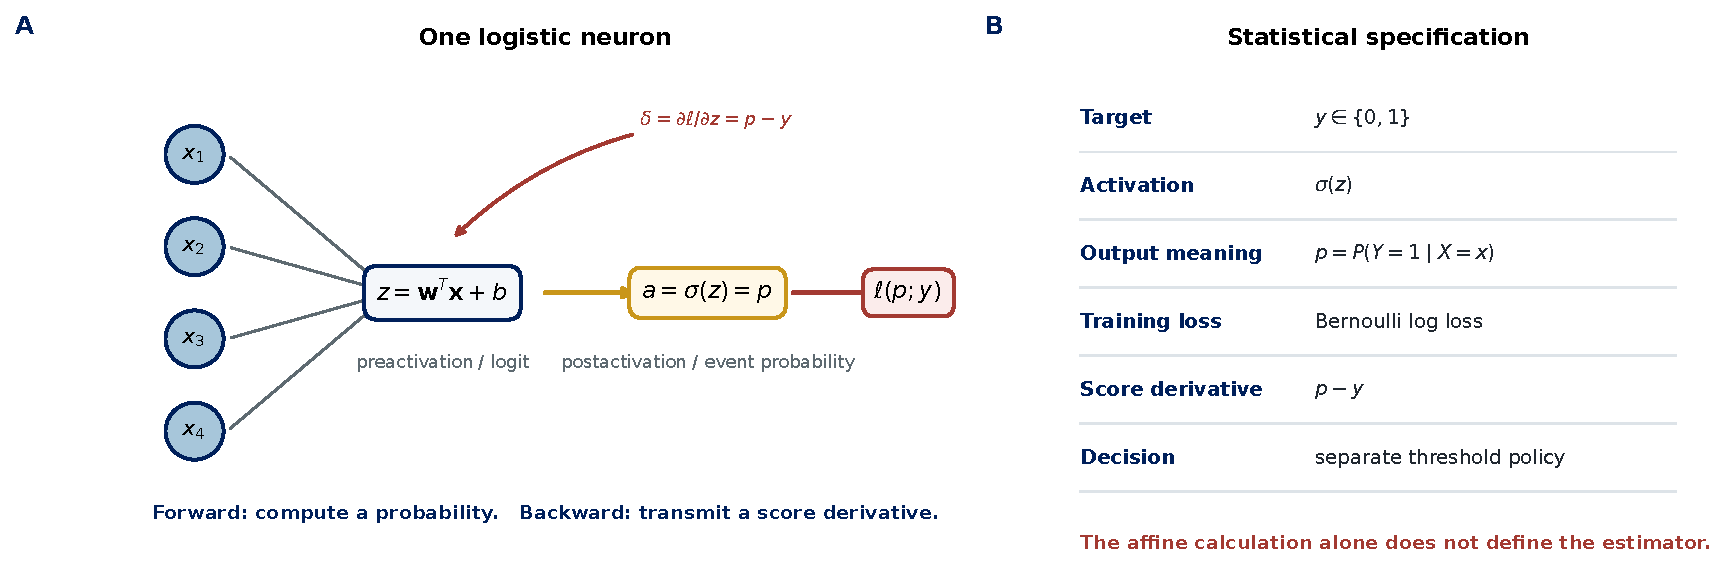
\includegraphics[width=\textwidth]{figures/generated/logistic-single-neuron.pdf}
  \caption{The logistic single-neuron contract. \textbf{A:} A forward pass
  forms the preactivation $z=w^Tx+b$ and the postactivation
  $a=\sigma(z)=p$. Bernoulli log loss returns the score derivative
  $\delta=\partial\ell/\partial z=p-y$ during the backward calculation.
  \textbf{B:} The computational graph becomes a statistical estimator only
  after its target, activation, loss, output meaning, and decision boundary are
  specified.}
  \label{fig:logistic-single-neuron}
\end{figure}

Figure~\ref{fig:logistic-single-neuron} is also a map of the derivation ahead.
The sigmoid supplies the probability range, the Bernoulli likelihood supplies
the loss, and the chain rule supplies the backward signal $p-y$.

\section{The sigmoid turns a score into a probability}

The logistic sigmoid is
\[
\sigma(z)=\frac{1}{1+e^{-z}}.
\]
It is not merely a convenient S-shaped curve. It is an invertible map from the
real line to the open unit interval and therefore connects an unconstrained
linear score with a valid probability.

\begin{proposition}[basic sigmoid geometry]
For every $z\in\mathbb{R}$,
\[
0<\sigma(z)<1,
\qquad
\sigma(0)=\frac12,
\qquad
\sigma(-z)=1-\sigma(z),
\qquad
\sigma'(z)=\sigma(z)\bigl(1-\sigma(z)\bigr).
\]
The derivative is positive and is maximized at $z=0$, where
$\sigma'(0)=1/4$.
\end{proposition}

\begin{proof}
The denominator $1+e^{-z}$ exceeds one, which gives the range. Substitution
gives $\sigma(0)=1/2$. Multiplying numerator and denominator by $e^z$ gives
$\sigma(z)=e^z/(1+e^z)$, from which the symmetry identity follows. Direct
differentiation yields
\[
\sigma'(z)=\frac{e^{-z}}{(1+e^{-z})^2}
=\sigma(z)\bigl(1-\sigma(z)\bigr).
\]
Writing $u=\sigma(z)\in(0,1)$ reduces the derivative to $u(1-u)$, a concave
quadratic with its unique maximum $1/4$ at $u=1/2$, equivalently $z=0$.
\end{proof}

For one feature $x$, let $z=b+wx$. If $w\ne0$, then
\[
p(x)=\sigma(b+wx)
=\sigma\!\left(w(x-x_{0.5})\right),
\qquad
x_{0.5}=-\frac{b}{w}.
\]
The midpoint $x_{0.5}$ is the feature value at which $p(x)=1/2$. The sign of
$w$ determines whether the curve rises or falls. Its magnitude controls the
steepness on the chosen feature scale, and
\[
\left.\frac{dp}{dx}\right|_{x=x_{0.5}}=\frac{w}{4}.
\]
Thus the numerical coefficient depends on units. If millimeters become meters,
the stored preprocessing and the coefficient must change together.

\begin{figure}[htbp]
  \centering
  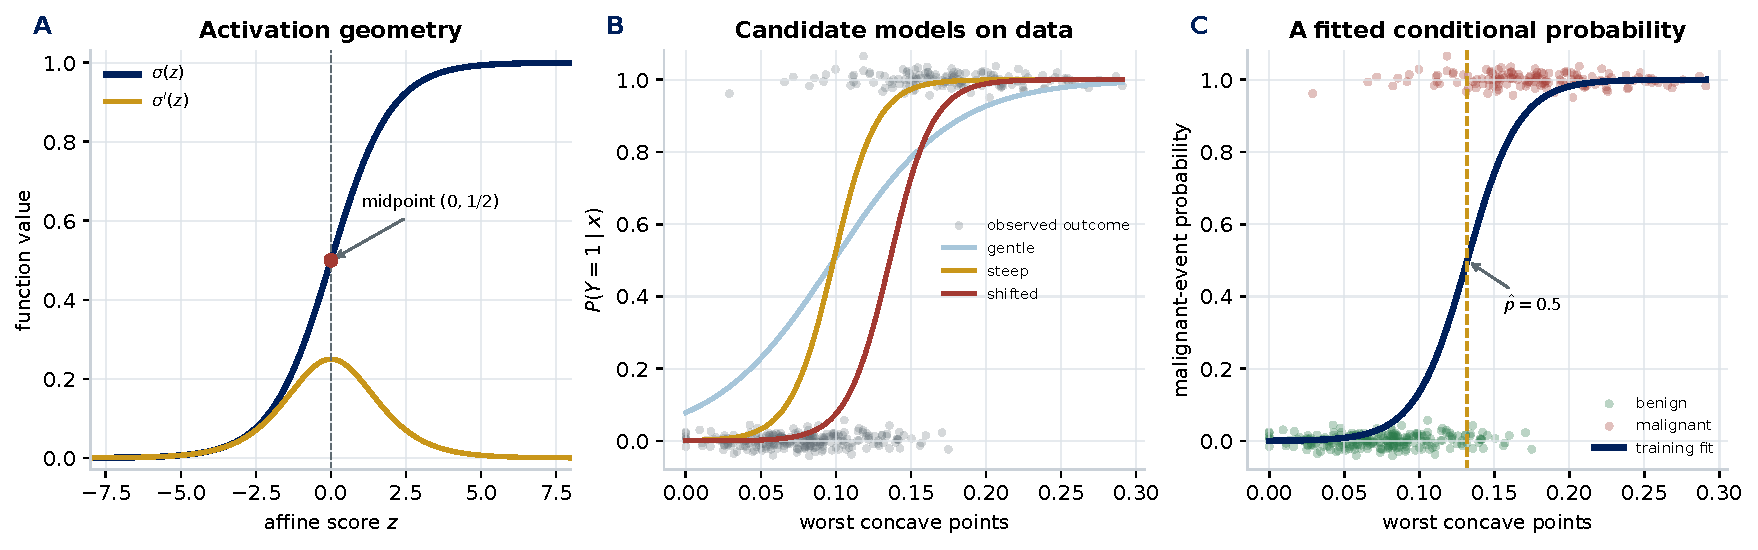
\includegraphics[width=\textwidth]{figures/generated/logistic-sigmoid-data.pdf}
  \caption{From activation to data. \textbf{A:} The sigmoid maps every real
  score to $(0,1)$; its derivative is largest at the midpoint and vanishes in
  the saturated tails. \textbf{B:} Several sigmoid curves can be placed over
  the same binary observations, so shape must be learned rather than selected
  by eye. \textbf{C:} A one-feature logistic model fitted on a training split of
  the Wisconsin Diagnostic Breast Cancer data produces a conditional
  malignant-event probability. Vertical jitter only reveals overlapping binary
  outcomes; it is not a new response value.}
  \label{fig:logistic-sigmoid-data}
\end{figure}

Figure~\ref{fig:logistic-sigmoid-data} makes a subtle point visible: an observed
binary response does not lie on the fitted curve except in the limiting sense
of zero or one. The curve estimates the conditional mean of the Bernoulli
outcome. Many observations near the same $x$ would be needed to estimate that
mean directly; the logistic form shares information across feature values.

\subsection{Odds and log-odds}

For $0<p<1$, the \term{odds} of the event are $p/(1-p)$. The inverse sigmoid
satisfies
\[
\operatorname{logit}(p)=\log\frac{p}{1-p}.
\]
The logistic-regression model is therefore
\[
\log\frac{p(x)}{1-p(x)}=w^Tx+b.
\]
Holding all other features fixed, increasing feature $x_j$ by one unit adds
$w_j$ to the log-odds and multiplies the odds by $e^{w_j}$. This is an
associational model statement, not a causal effect. Correlated features,
measurement choices, selection, and interventions all require additional
reasoning.

\begin{misconceptionbox}
\textbf{Misconception:} a coefficient of $0.7$ increases probability by $0.7$.
\textbf{Correction:} it multiplies the conditional odds by $e^{0.7}$ when the
other recorded features are held fixed. The probability change depends on the
starting probability because the sigmoid is nonlinear.
\end{misconceptionbox}

\section{Likelihood turns probability modeling into estimation}

Probability and likelihood use the same formula in different directions.
Probability holds a parameter fixed and studies possible outcomes. Likelihood
holds the observed outcomes fixed and compares candidate parameter values.

For conditionally independent observations, the Bernoulli likelihood is
\[
L(w,b;y_1,\ldots,y_n)
=\prod_{i=1}^n
p_i^{y_i}(1-p_i)^{1-y_i},
\qquad
p_i=\sigma(w^Tx_i+b).
\]
Conditional independence is an assumption. Repeated measurements from one
patient, neighboring pixels, related financial accounts, or time-adjacent
sensor readings may violate it. The split design must respect the dependence
unit even when the optimization code accepts rows independently.

Products of many probabilities become numerically tiny. Taking a logarithm
converts the product into a sum without changing its maximizer. Negating and
averaging gives the empirical logistic loss
\[
J(w,b)
=-\frac1n\sum_{i=1}^n
\left[y_i\log p_i+(1-y_i)\log(1-p_i)\right].
\]
For one observation,
\[
\ell(p;y)=-y\log p-(1-y)\log(1-p).
\]
When $y=1$, the loss is $-\log p$; when $y=0$, it is $-\log(1-p)$. A confident
wrong probability receives an unbounded penalty.

\begin{figure}[htbp]
  \centering
  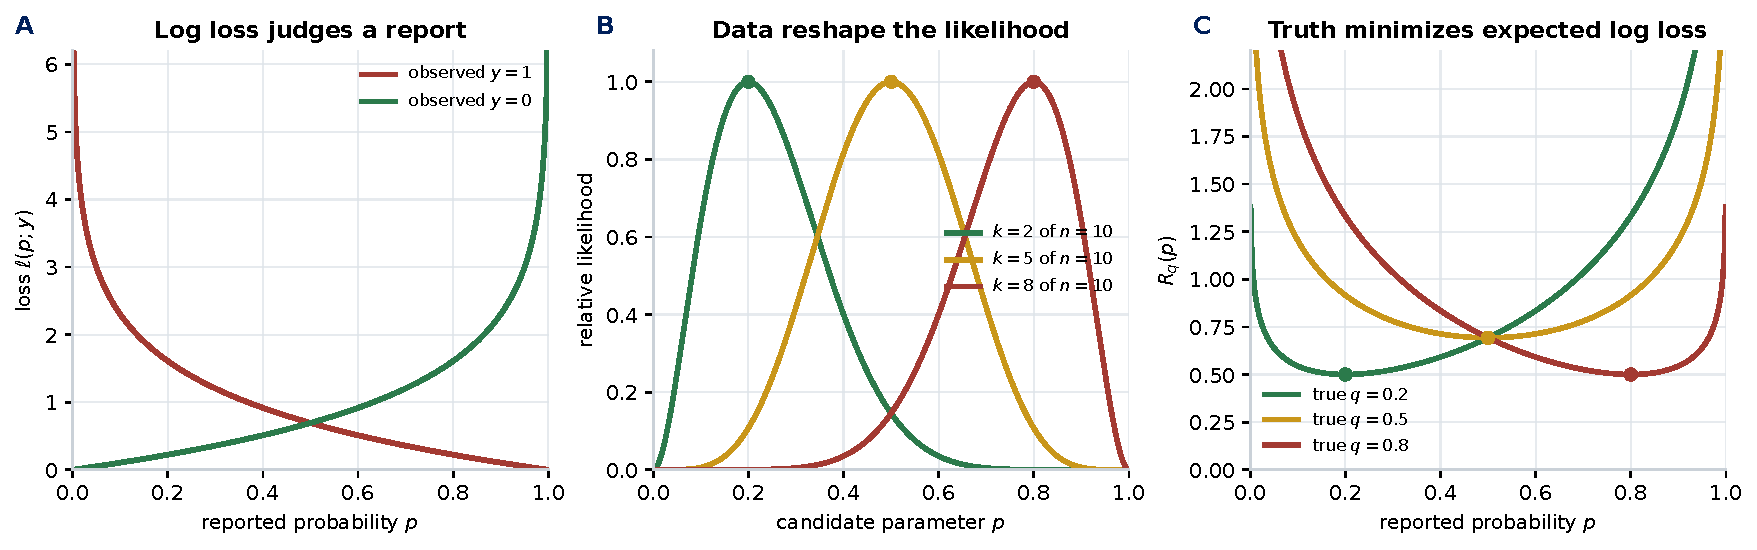
\includegraphics[width=\textwidth]{figures/generated/logistic-loss-geometry.pdf}
  \caption{Three views of the Bernoulli model. \textbf{A:} Per-observation log
  loss rewards probability assigned to the observed outcome and sharply
  penalizes confident errors. \textbf{B:} With $k$ events in ten trials, the
  likelihood is maximized at $\widehat p=k/10$; its width records finite-sample
  uncertainty. Curves are normalized only for visual comparison. \textbf{C:}
  If the true event probability is $q$, expected log loss is uniquely minimized
  by reporting $p=q$.}
  \label{fig:logistic-loss-geometry}
\end{figure}

\subsection{Why log loss elicits a probability}

A loss for probability forecasts should not reward systematic exaggeration or
hedging. Log loss has this property.

\begin{theorem}[strict propriety of Bernoulli log loss]
Let $Y\sim\operatorname{Bernoulli}(q)$ with $q\in(0,1)$. If a forecaster reports
$p\in(0,1)$, its expected log loss is
\[
R_q(p)=-q\log p-(1-q)\log(1-p).
\]
The unique minimizer is $p=q$.
\end{theorem}

\begin{proof}
Differentiate with respect to the reported probability:
\[
R_q'(p)=-\frac{q}{p}+\frac{1-q}{1-p}
=\frac{p-q}{p(1-p)}.
\]
The denominator is positive on $(0,1)$, so the derivative is negative for
$p<q$, zero at $p=q$, and positive for $p>q$. Equivalently,
\[
R_q(p)-R_q(q)
=D_{\mathrm{KL}}\!\left(
\operatorname{Bernoulli}(q)\,\Vert\,\operatorname{Bernoulli}(p)
\right)\ge0,
\]
with equality only when $p=q$.
\end{proof}

The theorem is a population statement. It does not guarantee that the chosen
feature representation and affine log-odds can express the true conditional
probability $q(x)$. Nor does it guarantee that the training population matches
deployment. A proper loss encourages honest reporting within the model and data
available; it cannot repair misspecification or distribution shift.

\conceptcheck{Why does 100 percent training accuracy fail to establish that the
reported probabilities are meaningful? Give one optimization reason and one
data-generating reason.}

\section{The gradient reveals the single-neuron connection}

Write the augmented design matrix and parameter vector as
\[
\widetilde X=
\begin{bmatrix}
1 & x_1^T\\
\vdots & \vdots\\
1 & x_n^T
\end{bmatrix},
\qquad
\theta=\begin{bmatrix}b\\w\end{bmatrix},
\qquad
z=\widetilde X\theta,
\qquad
p=\sigma(z).
\]
The model is a single computational unit: an affine score followed by a sigmoid
activation. The loss, rather than the picture of the unit, determines the
learning rule.

\begin{theorem}[logistic-loss gradient and Hessian]
For the average Bernoulli negative log-likelihood,
\[
\nabla_\theta J(\theta)=\frac1n\widetilde X^T(p-y)
\]
and
\[
\nabla_\theta^2J(\theta)
=\frac1n\widetilde X^T W\widetilde X,
\qquad
W=\operatorname{diag}\!\bigl(p_i(1-p_i)\bigr).
\]
Consequently, $J$ is convex.
\end{theorem}

\begin{proof}
For one row, use $p_i=\sigma(z_i)$ and
$dp_i/dz_i=p_i(1-p_i)$. The chain rule gives
\[
\frac{\partial\ell_i}{\partial z_i}
=\left(-\frac{y_i}{p_i}+\frac{1-y_i}{1-p_i}\right)
p_i(1-p_i)
=p_i-y_i.
\]
Since $\nabla_\theta z_i=\widetilde x_i$, summing and averaging yields the
gradient. Differentiating once more gives the stated Hessian. For every vector
$v$,
\[
v^T\nabla^2J(\theta)v
=\frac1n(\widetilde Xv)^TW(\widetilde Xv)\ge0,
\]
because every diagonal entry of $W$ is nonnegative. Hence the Hessian is
positive semidefinite and $J$ is convex.
\end{proof}

In the computational notation introduced earlier, $a=p$, so the backward
signal can be written either as $p-y$ or $a-y$. The probability notation is
preferable here because it prevents the output's statistical meaning from
disappearing. The residual-like term makes the update resemble linear
regression:
\[
\theta_{t+1}
=\theta_t-\eta\frac1n\widetilde X^T(p_t-y).
\]
But the resemblance must not erase the differences. Linear regression usually
uses an identity response map and squared error; logistic regression uses a
sigmoid response map and Bernoulli log loss. Its curvature changes with the
current probabilities through $W$.

Convexity means that any finite stationary point is globally optimal. It does
not mean that every implementation converges, that the optimum is unique, or
that the fitted probability generalizes. If the data are perfectly separable,
the unregularized likelihood may improve as $\lVert w\rVert\to\infty$ without
attaining a finite minimizer.

\section{Stable computation is part of the mathematics}

The expression $\log(1+e^z)$ overflows when $z$ is large. NumPy names the
stable two-argument operation
\[
\operatorname{logaddexp}(a,b) := \log\!\left(e^a+e^b\right).
\]
Consequently,
$\operatorname{logaddexp}(0,z)=\log(e^0+e^z)=\log(1+e^z)$; the zero is the
first argument to the operation, not an extra term in the statistical model.
This gives the stable softplus form of the per-row loss:
\[
\ell(z;y)=\log(1+e^z)-yz
=\operatorname{logaddexp}(0,z)-yz.
\]
Implementations evaluate this quantity without first constructing the possibly
enormous value $e^z$---for example, as
$\max(0,z)+\log(1+e^{-|z|})$.
Likewise, a stable sigmoid evaluates positive and negative scores by different
algebraically equivalent branches.

\begin{lstlisting}[language=Python,caption={Stable scalar sigmoid and vectorized loss from logits.}]
def stable_sigmoid(score: float) -> float:
    """Map a real score to an event probability without overflow."""
    if score >= 0.0:
        return 1.0 / (1.0 + math.exp(-score))
    exponential = math.exp(score)
    return exponential / (1.0 + exponential)


def logistic_loss_from_logits(logits, outcomes):
    """Return mean Bernoulli negative log-likelihood from raw logits."""
    logits = np.asarray(logits, dtype=float)
    outcomes = np.asarray(outcomes, dtype=float)
    if logits.shape != outcomes.shape:
        raise ValueError("logits and outcomes must have the same shape")
    return np.mean(np.logaddexp(0.0, logits) - outcomes * logits)
\end{lstlisting}

A professional implementation tests values such as $z=\pm1000$, verifies an
analytic gradient against central finite differences, records termination
status, and compares a transparent implementation with an independent library.
The comparison must align regularization, intercept handling, feature scaling,
class order, tolerance, and stopping criteria. Agreement after those choices is
strong evidence; agreement by accident is not.

\begin{professionalbox}
Fit preprocessing and the estimator as one pipeline. Persist feature order,
units, target encoding, scaler state, model parameters, software versions, and
training-data identity. A coefficient vector without its preprocessing and
semantic contract is not a deployable model.
\end{professionalbox}

\section{A complete evidence workflow}

Logistic regression does not remove the evidence boundaries introduced in
Chapter~\ref{ch:supervised-contract}. A defensible workflow proceeds as follows:
\begin{enumerate}
  \item define the positive event, prediction unit, horizon, and deployment
  population;
  \item inspect schema, missingness, ranges, duplicates, dependence, and class
  prevalence;
  \item split by the real independence unit before fitting transformations;
  \item fit imputers, scalers, feature transformations, and the estimator on
  training data only;
  \item use validation data for model, regularization, and threshold choices;
  \item compare probability quality and decision utility with declared
  baselines; and
  \item open the sealed test set once for the frozen model-policy pair.
\end{enumerate}

Scaling is not required to make the logistic formula valid. It improves
optimization conditioning and makes regularization act more comparably across
features. Scaling the complete dataset before splitting is leakage because the
validation and test feature distributions influence the fitted transformation.

\subsection{Real-data example: diagnostic measurements}

\begin{workedexample}{diagnostic measurement to review policy}
The companion notebook reads the Wisconsin Diagnostic Breast Cancer table from
the repository's SQLite database. It defines
\[
Y=\mathbf{1}\{\text{diagnosis is malignant}\}.
\]
This dataset is appropriate for learning estimation and evaluation, but it is
not a clinical validation study and the resulting model must not be described
as a medical device.

A regularized pipeline fits scaling and logistic regression on training rows.
Validation rows then answer three separate questions: whether event and
non-event probabilities separate, whether reported probabilities agree with
observed frequencies, and which threshold serves one declared cost model. The
sealed test set remains unused until the model and policy are frozen.
\end{workedexample}

Figure~\ref{fig:logistic-validation-evidence} fits a regularized logistic
pipeline on a training split and uses a validation split for three different
questions. The panels intentionally do not collapse into one ``model quality''
number.

\begin{figure}[htbp]
  \centering
  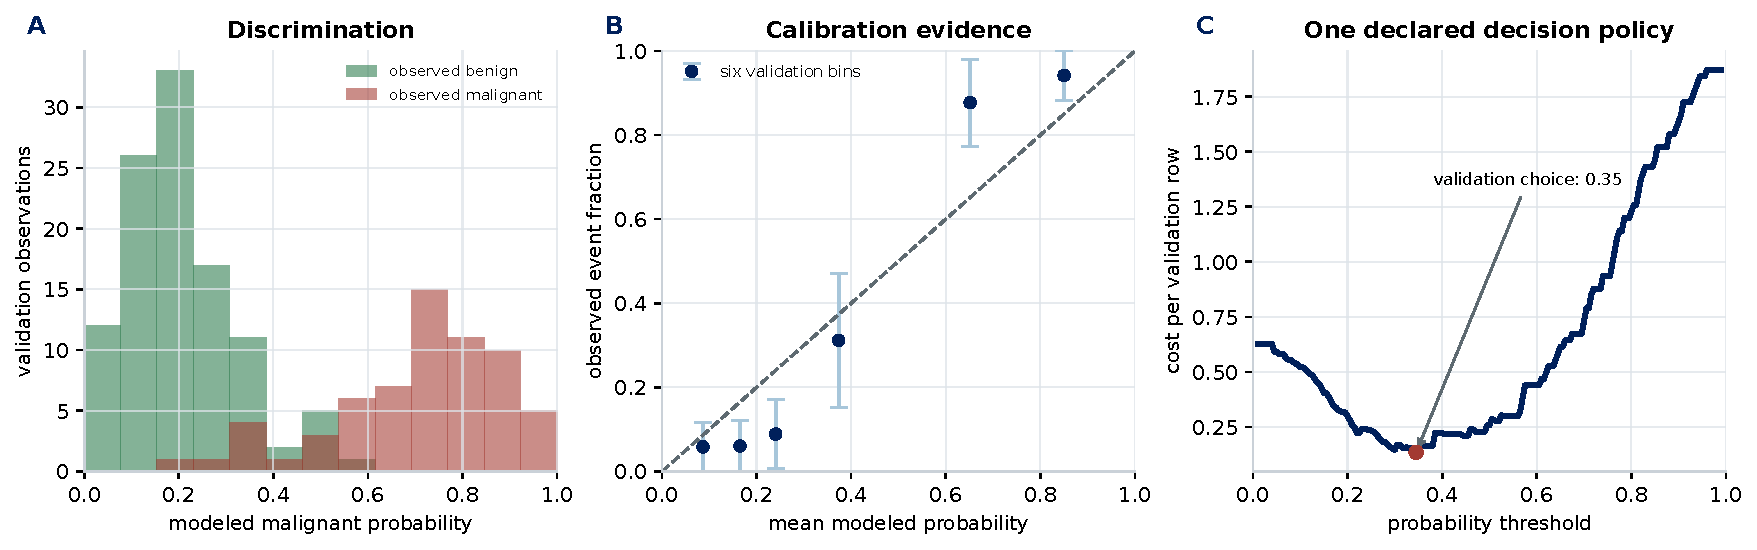
\includegraphics[width=\textwidth]{figures/generated/logistic-validation-evidence.pdf}
  \caption{Three forms of validation evidence from the repository's breast
  cancer table. \textbf{A:} Class-conditional probability histograms describe
  discrimination. \textbf{B:} Binned event fractions with 95 percent Wilson
  intervals provide limited calibration evidence; the intervals expose the
  small validation sample. \textbf{C:} A threshold is chosen for one explicitly
  hypothetical cost model in which a false negative costs five times a false
  positive. Changing that cost model can change the action rule without
  changing the fitted probability model.}
  \label{fig:logistic-validation-evidence}
\end{figure}

\section{Measuring classification performance professionally}

``How accurate is the model?'' is not a complete evaluation question. A
professional report first names the claim, population, sample, baseline, and
decision policy. It then measures several properties because classification
performance has at least three layers.

\begin{itemize}
  \item \textbf{Probability quality:} Did the model assign useful probabilities
  to what occurred? Examine log loss, Brier score, and calibration evidence.
  \item \textbf{Discrimination:} Do event cases tend to rank above non-event
  cases? Examine ROC and precision-recall curves and their summaries.
  \item \textbf{Decision performance:} What happened under one specified action
  rule? Examine confusion counts, conditional rates, cost, and capacity.
\end{itemize}

No layer replaces the others. A model can rank cases well while systematically
overstating probability. A well-calibrated model can still serve a poor action
policy. A high-accuracy policy may merely predict the common class.

\subsection{Begin with a baseline and probability evidence}

The average validation log loss measures the probability assigned to observed
outcomes. The Brier score
\[
\frac1m\sum_{i=1}^m(p_i-y_i)^2
\]
is another proper score. Both should be compared with a baseline fitted without
test information. A prevalence baseline reports the training event frequency
for every row. In an operational study, the relevant baseline might instead be
the current laboratory workflow, an established score, or a policy that sends
every case for review. A complex model that cannot improve on the relevant
baseline has not earned its complexity.

\term{Discrimination} asks whether event rows tend to receive larger scores
than non-event rows. ROC AUC is the probability that a randomly selected event
row receives a higher score than a randomly selected non-event row, with
standard handling for ties. It is threshold-free and does not establish
calibration. Precision-recall summaries are sensitive to event prevalence and
can be more informative for rare events.

\term{Calibration} asks whether probabilities mean what they report on a stated
population. Among comparable cases assigned probability near $q$, an event rate
near $q$ supports calibration. Reliability diagrams depend on binning and sample
size, so uncertainty must be visible. A sigmoid output is constrained to
$(0,1)$, but range is not calibration.

\begin{misconceptionbox}
\textbf{Misconception:} a high ROC AUC proves that probabilities are accurate.
\textbf{Correction:} any strictly increasing transformation preserves ranking
and therefore ROC AUC while changing probability values. Calibration requires
separate evidence.
\end{misconceptionbox}

Calibration may drift when prevalence, measurement, or case mix changes.
Post-hoc methods such as Platt scaling or isotonic regression must be fitted on
data not used to fit the underlying score, commonly through cross-validated or
nested procedures. Recalibration is an estimated model, not a cosmetic plotting
operation.

\subsection{A confusion matrix is four counts with four meanings}

After a threshold $t$ defines
$\widehat Y=\mathbf{1}\{p\ge t\}$, every evaluated row enters one cell:

\begin{center}
\begin{tabular}{@{}lcc@{}}
\toprule
& Predicted non-event & Predicted event \\
\midrule
Actual non-event & true negative (TN) & false positive (FP) \\
Actual event & false negative (FN) & true positive (TP) \\
\bottomrule
\end{tabular}
\end{center}

The word ``positive'' identifies the declared event; it does not mean a good
outcome. The word ``false'' means that the thresholded action disagrees with the
recorded label. It does not establish that the label, measurement process, or
sampling design is correct.

Several familiar rates use different conditioning sets:
\[
\operatorname{sensitivity}
=\frac{TP}{TP+FN}=P(\widehat Y=1\mid Y=1),
\qquad
\operatorname{specificity}
=\frac{TN}{TN+FP}=P(\widehat Y=0\mid Y=0),
\]
\[
\operatorname{precision}
=\frac{TP}{TP+FP}=P(Y=1\mid\widehat Y=1),
\qquad
\operatorname{NPV}
=\frac{TN}{TN+FN}=P(Y=0\mid\widehat Y=0).
\]
Sensitivity conditions on actual event rows; precision conditions on predicted
event actions. Interchanging them reverses a conditional probability. False
positive rate is $FP/(FP+TN)=1-\text{specificity}$, and false negative rate is
$FN/(FN+TP)=1-\text{sensitivity}$. Balanced accuracy averages sensitivity and
specificity so that the more common class does not dominate the average.

Always report the four counts with the rates. A sensitivity of 90 percent based
on 18 of 20 event rows and one based on 18,000 of 20,000 rows are the same point
estimate but not the same amount of evidence. A zero denominator makes the
corresponding rate undefined, not zero.

\subsection{The evaluated data determine what a metric means}

Let event prevalence be $\pi=P(Y=1)$, sensitivity be $s$, and specificity be
$c$. Even if $s$ and $c$ transported unchanged to a new population,
\[
\operatorname{precision}
=\frac{\pi s}{\pi s+(1-\pi)(1-c)},
\qquad
\operatorname{accuracy}=\pi s+(1-\pi)c.
\]
Precision and accuracy therefore change when the event prevalence changes.
This is not a defect in the formulas; it records a change in the question being
asked of the system.

\begin{figure}[htbp]
  \centering
  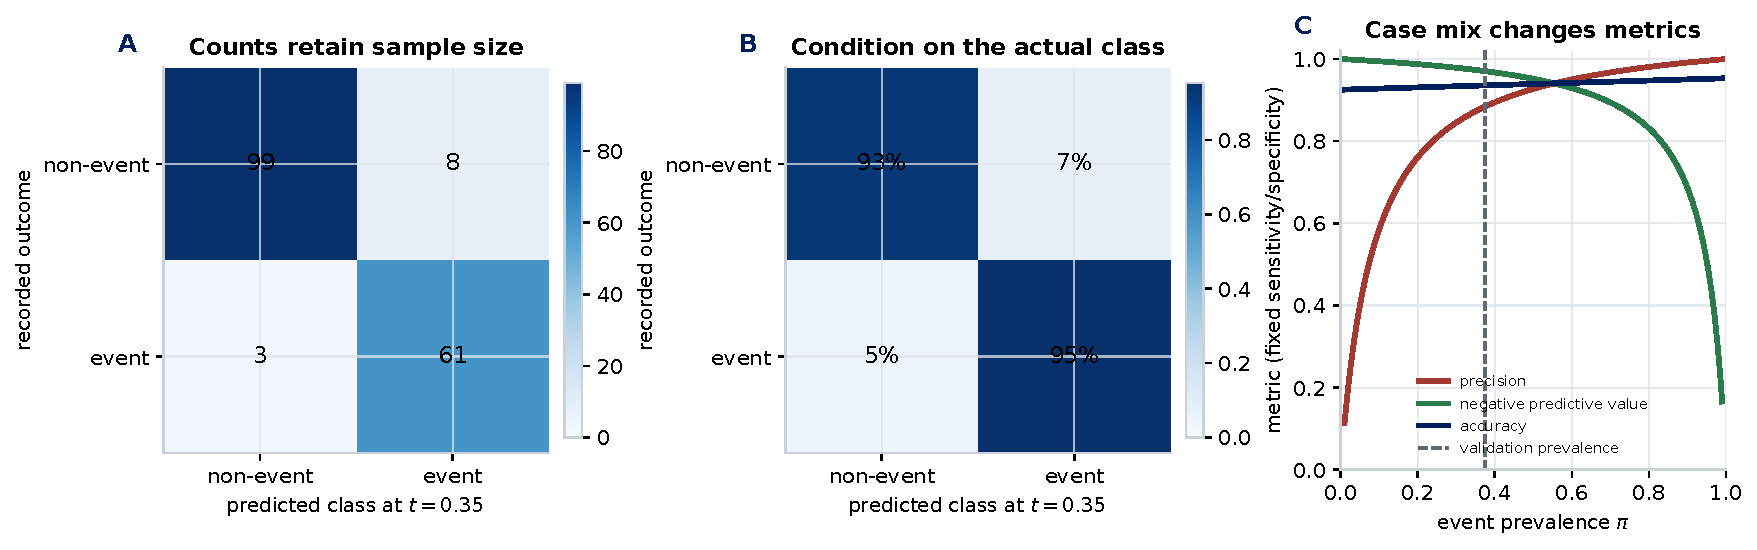
\includegraphics[width=\textwidth]{figures/generated/classification-performance-context.pdf}
  \caption{A confusion matrix is contextual evidence, not a permanent model
  attribute. \textbf{A:} Counts retain the validation sample size at the
  threshold selected under the explicitly hypothetical five-to-one error cost.
  \textbf{B:} Row normalization conditions on the recorded actual class and
  exposes sensitivity and specificity. \textbf{C:} Holding those two rates fixed
  while changing prevalence still changes precision, negative predictive value,
  and accuracy. The vertical line marks only this validation sample's
  prevalence; it is not a deployment estimate.}
  \label{fig:classification-performance-context}
\end{figure}

Prevalence is only one aspect of data context. Performance can also change with
disease severity, sensor calibration, laboratory site, acquisition protocol,
missingness, time, demographic composition, treatment access, and the definition
or quality of the outcome label. A dataset with easier, more extreme cases may
produce stronger discrimination than a screening population with subtle cases.
This broader dependence on the range and mix of cases is often called
\term{spectrum effect}.

The repository's breast-cancer table is not a random sample of every future
clinical case. Its prevalence must not be substituted for that of a hospital,
screening program, or community. It also lacks the site, time, demographic, and
workflow variables needed for an external-validity or subgroup audit. The
professional response is to name that evidence gap, not to hide it behind an
aggregate score.

\conceptcheck{A classifier has the same sensitivity and specificity at two
hospitals but much lower precision at one. Give a mathematical explanation and
two data-quality explanations that should be investigated.}

\subsection{Attach uncertainty and scope to every performance claim}

Validation metrics are estimates from a finite sample. For a frozen model and
threshold, a binomial interval may summarize uncertainty in sensitivity or
specificity when observations are independent. If rows are grouped by patient,
site, batch, or time, resampling and intervals must preserve those groups.
Repeated cross-validation can study development variability, but it does not
turn adaptively reused data into an untouched final test set.

A professional classification report records:
\begin{itemize}
  \item event definition, horizon, prediction unit, intended use, and target
  population;
  \item dataset sources, dates, sites, inclusion rules, sample sizes, and
  prevalence;
  \item split unit, baselines, and every model-selection decision;
  \item log loss or Brier score, discrimination, and calibration evidence;
  \item the versioned threshold, confusion counts, conditional rates, costs,
  capacity, and uncertainty intervals;
  \item performance by relevant site, time period, and subgroup, together with
  the sample size of every slice;
  \item known missing slices, label limitations, and plausible deployment
  shifts; and
  \item model, feature, software, data, and policy versions sufficient to
  reproduce the report.
\end{itemize}

\section{A probability model is not a decision policy}

Let action $a=1$ mean ``intervene'' and $a=0$ mean ``do not intervene.'' Suppose
a false positive costs $C_{FP}>0$ and a false negative costs $C_{FN}>0$, while
correct actions have zero cost. Given a calibrated probability $p$, the
conditional risks are
\[
R(a=1\mid x)=C_{FP}(1-p),
\qquad
R(a=0\mid x)=C_{FN}p.
\]

\begin{proposition}[cost-sensitive threshold]
Under the stated two-action cost model, choose action $1$ exactly when
\[
p\ge \frac{C_{FP}}{C_{FP}+C_{FN}}.
\]
\end{proposition}

\begin{proof}
Choose action $1$ when its conditional risk is no larger:
$C_{FP}(1-p)\le C_{FN}p$. Rearranging gives the stated threshold.
\end{proof}

The familiar threshold $0.5$ is optimal only under this simplified model with
equal error costs. Real policies may include review capacity, delayed outcomes,
abstention, several actions, legal constraints, subgroup harms, or utilities
that vary by case. Threshold selection is therefore a product decision backed
by statistical evidence, not a default supplied by the sigmoid.

At every candidate threshold, recompute the confusion counts, conditional rates,
action volume, and operational cost. A threshold that exceeds review capacity is
not usable merely because it has attractive sensitivity. Conversely, a capacity
constraint is a property of the operating system, not a reason to relabel the
result as intrinsic model performance.

Version the decision policy separately from the score model. Costs, prevalence,
or capacity may change the threshold without requiring new model parameters.
Evaluate the final frozen model-policy pair on untouched test data.

\begin{warningbox}
Selecting a threshold on the test set converts the test set into validation
data. Reporting that same performance as final evidence is optimistic, even if
the model coefficients were never refitted.
\end{warningbox}

\section{Multiclass and multilabel extensions}

For $K$ mutually exclusive classes, a softmax converts logits $z_k$ into
\[
p_k=\frac{e^{z_k}}{\sum_{j=1}^K e^{z_j}},
\qquad
\sum_{k=1}^K p_k=1.
\]
Categorical cross-entropy is the corresponding negative log-likelihood. Stable
implementations subtract the largest logit or use a log-sum-exp primitive.

One-vs-rest fits $K$ binary problems and may require probability reconciliation.
Multilabel prediction is different: several labels may be true at once, so
independent sigmoid outputs may be appropriate. The data-generating semantics,
not the number of output columns, determine the model.

Macro averages weight classes equally; micro averages weight individual
decisions equally. Neither should replace class-level errors and an inspected
confusion matrix.

\section{Engineering the model as a reliable component}

A production classifier should expose explicit interfaces such as
\code{predict\_logit}, \code{predict\_proba}, and a separately versioned
\code{decide}. Tests should cover:
\begin{itemize}
  \item schema, feature order, units, missing values, and unexpected categories;
  \item positive-class identity and library \code{classes\_} ordering;
  \item finite output and $0\le p\le1$ at extreme inputs;
  \item agreement of analytic and numerical gradients;
  \item preprocessing fitted only on training rows;
  \item deterministic splits and reproducible optimization;
  \item threshold equality, abstention boundaries, and policy versions; and
  \item serialization round trips that preserve probabilities.
\end{itemize}

Monitoring must also preserve the distinctions in this chapter. Service logs
can immediately reveal latency, missing features, probability distributions,
and action rates. Discrimination and calibration require outcomes, which may
arrive later or only for a selected subset. A monitoring design must specify how
predictions are joined to outcomes and how selection bias enters that join.

\begin{professionalbox}
An API should not return a floating-point field called \code{risk} without a
contract. Document the event, horizon, applicable population, model version,
and probability semantics. If the API also returns an action, include the
policy version and enough trace information to reconstruct the decision.
\end{professionalbox}

\section{Exercises}

\subsection*{Conceptual and diagnostic problems}
\begin{enumerate}[label=\textbf{C\arabic*.}]
  \item A model returns a logit of $-2.3$. Explain why it is neither a
  probability nor a negative probability. Compute the corresponding event
  probability and odds.
  \item Explain why two observations with probabilities $0.51$ and $0.99$ have
  the same class prediction at threshold $0.5$ but provide different evidence.
  \item Give an example in which discrimination remains stable while
  calibration changes after deployment.
  \item A classifier has 99 percent accuracy on an event with prevalence
  1 percent. Construct a confusion matrix consistent with those facts but with
  zero recall.
  \item Distinguish the claims ``the event probability is 0.8,'' ``the model is
  80 percent confident,'' and ``80 percent of observed event rows have this
  measurement.'' Which claims are defined by logistic regression?
\end{enumerate}

\subsection*{Mathematical problems}
\begin{enumerate}[label=\textbf{M\arabic*.}]
  \item Derive $\sigma(-z)=1-\sigma(z)$ and use it to design a numerically stable
  implementation for both signs of $z$.
  \item Starting from the Bernoulli likelihood, derive the average negative
  log-likelihood without skipping the product-to-sum step.
  \item Derive the gradient with respect to $w$ and $b$ separately. Then recover
  the augmented-matrix formula.
  \item Prove that adding $\lambda\lVert w\rVert_2^2/2$ preserves convexity.
  State when the regularized objective is strictly convex.
  \item For the two-action cost model, derive the optimal threshold when correct
  positive and correct negative actions also have nonzero costs.
  \item Construct a linearly separable dataset and show analytically why scaling
  a separating parameter vector can drive unregularized logistic loss toward
  zero without reaching a finite minimizer.
\end{enumerate}

\subsection*{Computational investigations}
\begin{enumerate}[label=\textbf{P\arabic*.}]
  \item Query a binary dataset from the course SQLite database. Produce a data
  dictionary, prevalence report, missingness audit, and a split design tied to
  the independence unit.
  \item Implement stable sigmoid, loss, and gradient functions with NumPy-style
  docstrings and type hints. Test extreme logits and verify the gradient with
  central finite differences.
  \item Fit a transparent batch-gradient implementation and an unregularized
  library reference under matched conditions. Compare coefficients,
  probabilities, objective value, iterations, and wall time.
  \item Compare a prevalence baseline and a regularized pipeline using log loss,
  Brier score, ROC AUC, and a reliability diagram with uncertainty. Explain what
  each result does and does not establish.
  \item Specify two plausible cost models for one application. Show how the
  validation-selected threshold and confusion matrix change while model
  probabilities remain fixed.
\end{enumerate}

\subsection*{Contribution studio}

For contribution problem \textbf{CLF-PR1}, add a tested probability diagnostic
to the course package. The pull request must define the mathematical quantity,
include a failure-mode test, and demonstrate it on a public dataset without
opening the test split during development.

For contribution problem \textbf{CLF-PR2}, implement a regularized logistic
objective or reproducible benchmark recorder. Include typed public interfaces,
NumPy-style documentation, finite-difference verification, and evidence that
intercept treatment matches the written objective.

\begin{chapterreview}
Logistic regression is a conditional probability model built from an affine
score and the single-neuron computation $z=w^Tx+b$, $a=\sigma(z)=p$. Its
Bernoulli likelihood gives the backward signal $\delta=p-y$. The gradient
resembles the linear-regression gradient because both propagate a residual-like
signal through the same affine computation; the activation, response model,
loss, curvature, target domain, and interpretation are different. The next
model retains the affine score but replaces probabilities and log loss with
signed margins and hinge loss. Proper probability estimation, discrimination,
calibration, and decision utility remain separate forms of evidence. A reliable
system preserves those distinctions in code, evaluation, deployment, and
monitoring.
\end{chapterreview}

\begin{notebooklink}
Lecture 11 notebook 00 derives and fits the model, verifies its gradient, and
evaluates its evidence. Notebook 01 then studies the same affine skeleton under
the different semantics of a linear support vector machine. The following API
chapter unifies reusable mechanism only after those distinctions are explicit.
Production code belongs in tested modules.
\end{notebooklink}
